\chapter{TenderInsights}

\section{Kurze Projektbeschreibung}
In dem Projekt geht es darum einen PoC - also einen Proof of Concept zu erstellen, der mithilfe von AI bzw. Large Language 
Models (LLM) große Dokumente nach gesuchten Inhalten durchsucht und aufbereitet. Im Fokus stehen dabei insbesondere 
öffentliche Ausschreibungen zur Akquise von neuen Projekten für das Unternehmen. Bisher hat ein Mitarbeiter aus PMO die 
Ausschreibungen händisch grob für passend oder nicht geeignet erklärt und diese dann an die Akquise weitergeleitet. 
Dort hat ein Mitarbeiter die Ausschreibung sehr genau analysiert und einen sogenannten One Pager erstellt, der alle 
Daten welche für eine Entscheidung, ob man sich bewerben möchte oder nicht, relevant sind. Aufgabe des PoC ist es nun 
diesen One Pager mithilfe von künstlicher Intelligenz und einem LLM aus einer oder mehreren bereitgestellten PDF-Datei zu 
generieren. Der Anwender soll dies über ein Userinterface im Stile einer Webanwendung bedienen können.

\section{Verwendete Software}
In diesem Kapitel werden alle Software-Werkzeuge beschrieben, welche im Entwicklungsumfeld des TenderInsights verwendet werden.


\subsection{Technologien}

\begin{table}[H]
    \centering
    \caption{Übersicht der Technologien}
    \label{tab:technologien}
    \begin{tabular}{|l|l|}
    \hline
    \textbf{Name} & \textbf{Beschreibung} \\ \hline
    Name1 & Beschreibung1 \\ \hline
    Name2 & Beschreibung2 \\ \hline
    Name3 & Beschreibung3 \\ \hline
    \end{tabular}
\end{table}


\subsection{Werkzeuge}

\begin{table}[H]
    \centering
    \caption{Übersicht der Werkzeuge}
    \label{tab:werkzeuge}
    \begin{tabular}{|l|l|}
    \hline
    \textbf{Name} & \textbf{Beschreibung} \\ \hline
    Werkzeug1 & Beschreibung1 \\ \hline
    Werkzeug2 & Beschreibung2 \\ \hline
    Werkzeug3 & Beschreibung3 \\ \hline
    \end{tabular}
\end{table}



\begin{figure}[ht]
    \centering
    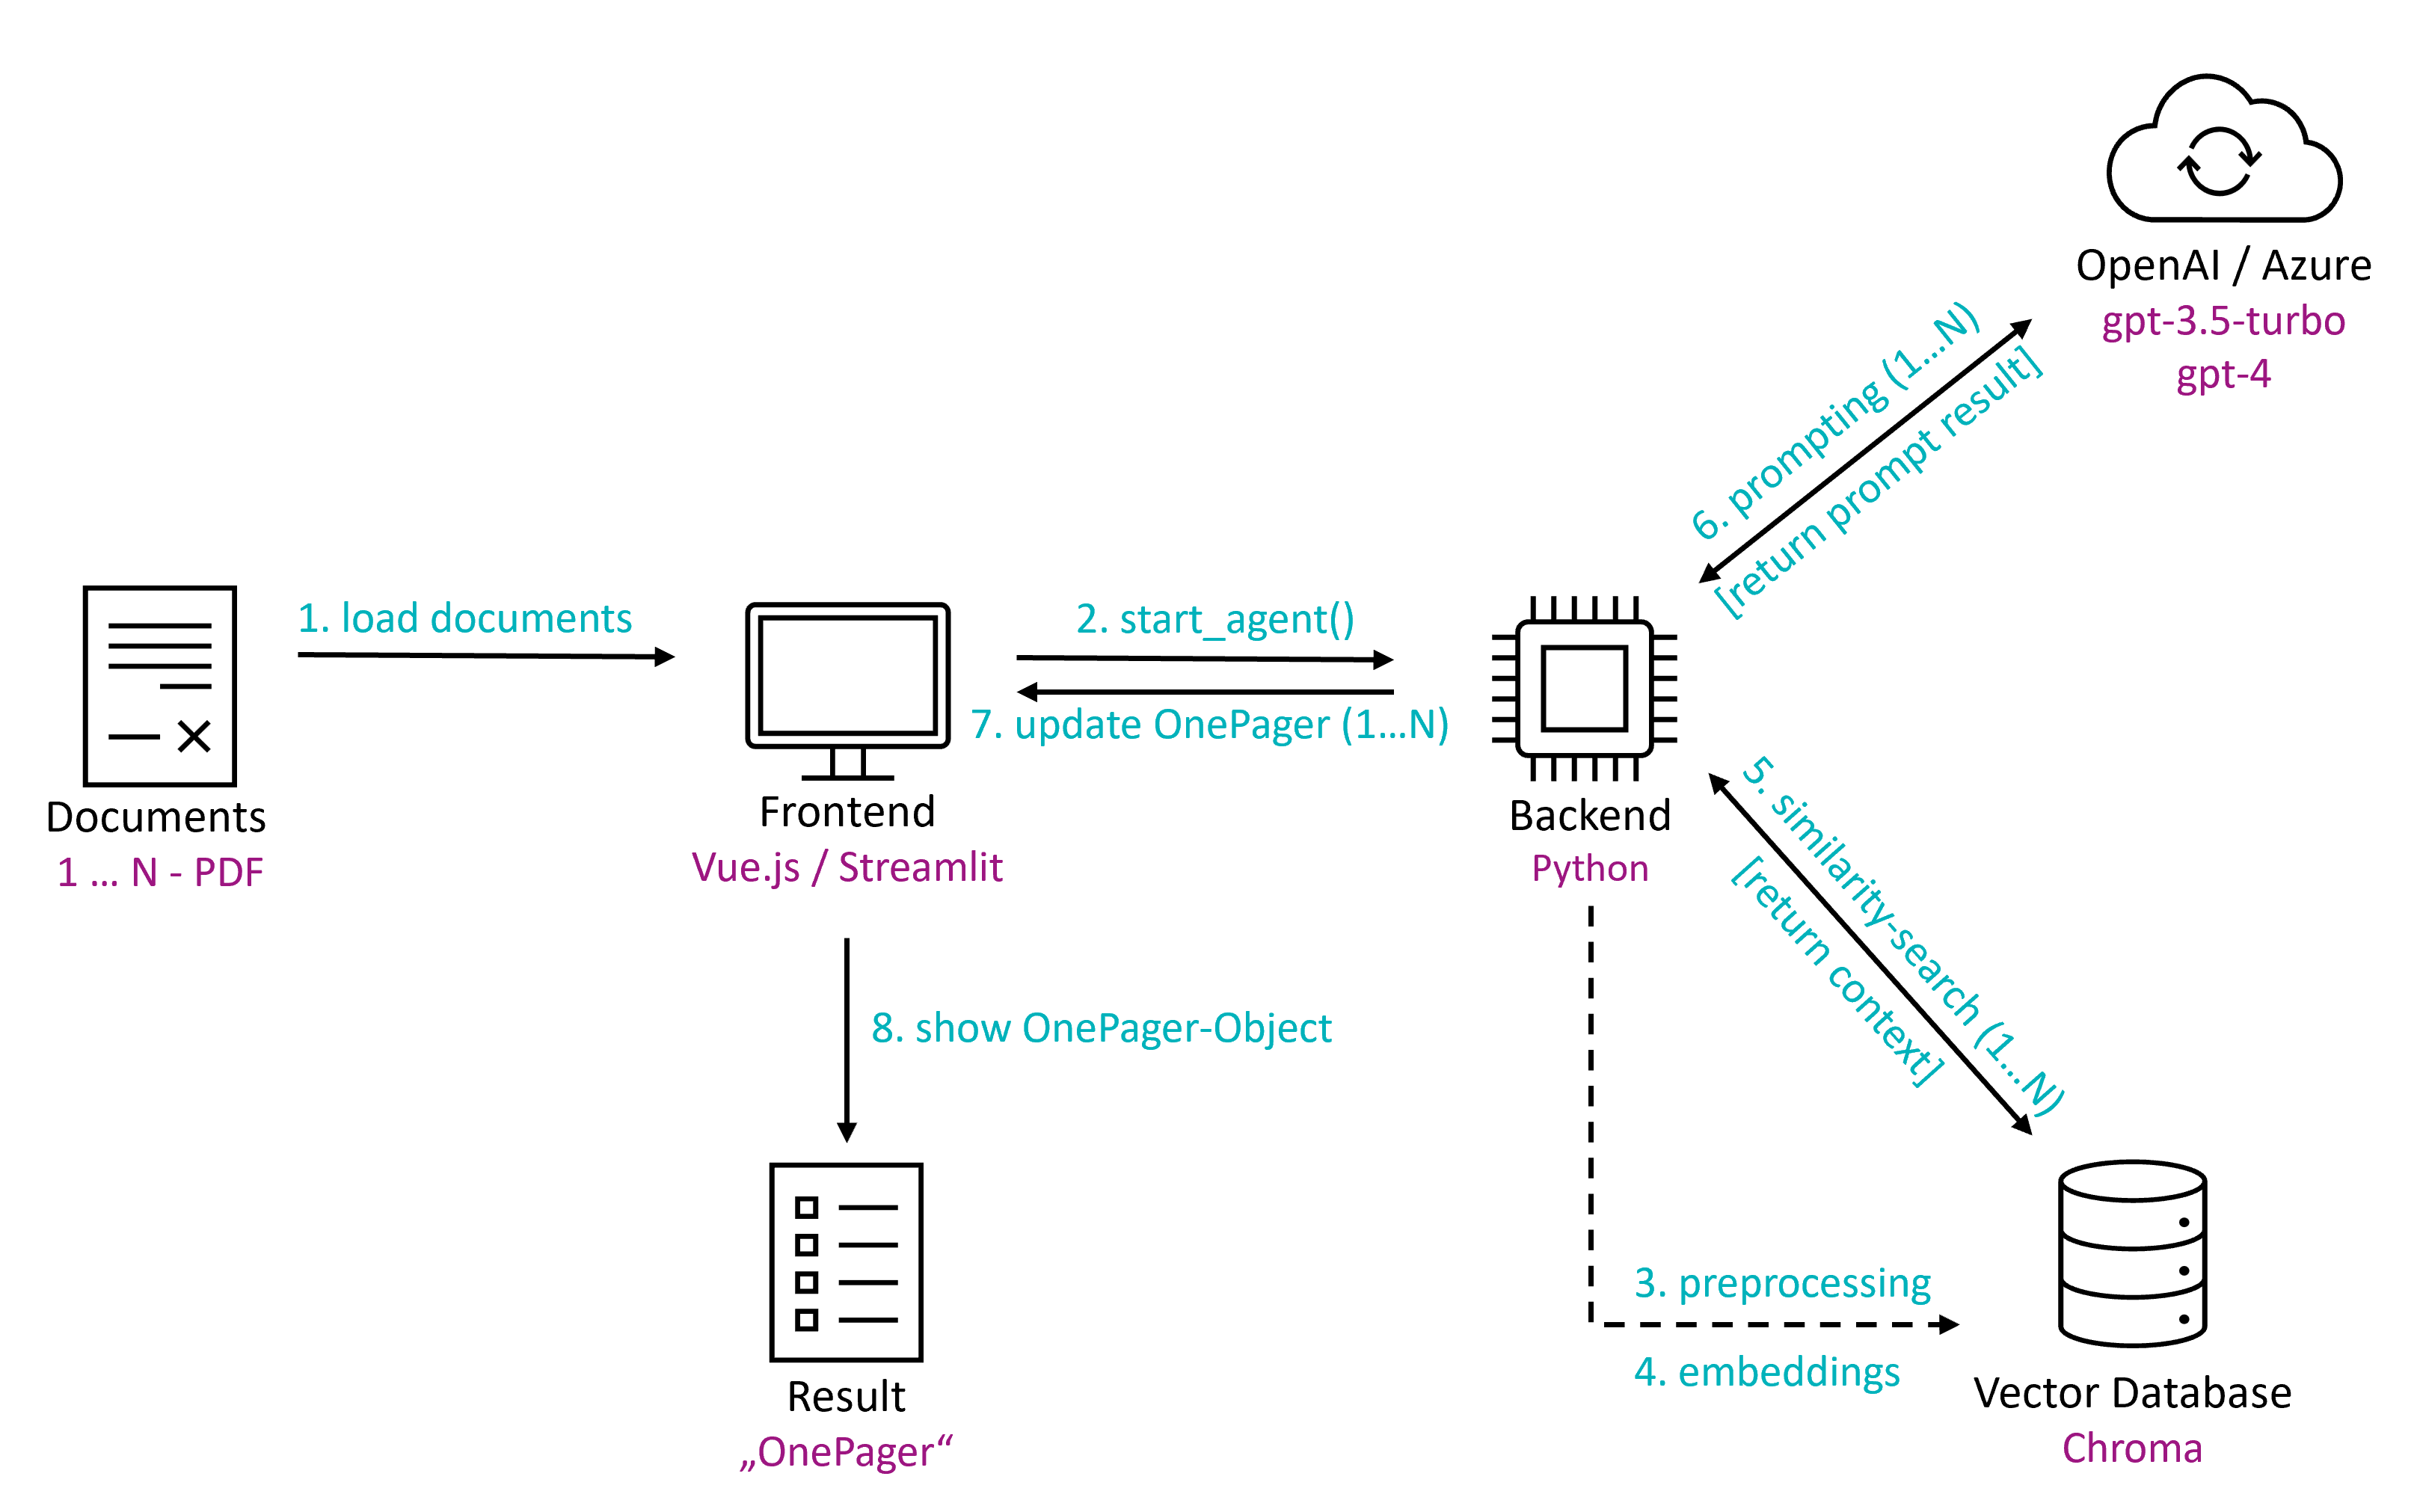
\includegraphics[width=0.8\textwidth]{figures/DokumentenAgent-Uebersicht.png}
    \caption{Schematische Darstellung der Software-Architektur}
    \label{fig:DokumentenAgent-uebersicht}    % \ref{fig:DokumentenAgent-uebersich}
\end{figure}


\section{Projektstand bei Arbeitsbeginn}
Zum Zeitpunkt meines Projekteintrittes gibt es bereits ein Frontend welches mithilfe von Streamlit implementiert wurde. 
PDF-Dateien können über einen File-Uploader im Frontend an die Anwendung übergeben werden. Da die meisten LLM-Modelle eine 
begrenzte Token-Anzahl für die Abfragen haben ist es nicht möglich das gesamte Dokument an das LLM zu übergeben. 
Daher wird das Dokument aufgesplittet und mittels einer Vektordatenbank auf Ähnlichkeit mit die gesuchte Information 
abgeglichen. Die k Ergebnisse mit der größten Ähnlichkeit werden zusammen mit dem Prompt als Abfrage an das LLM übermittelt. 
Die Abfragen werden mit der langchain API durchgführt, das verwendete Modell ist "gpt-3.5 turbo". 
Der Großteil dieser Funktionalitäten findet sich in der Document-Agent Klasse. Es gibt 3 Ausschreibungsdokumente in 
verschiedenen Größen mit denen die Abfragen getestet werden können. Es gibt 3 Prompts, welche bislang nur bedingt gute 
Ergebnisse liefern.

\section{Deine Rolle und Aufgaben im Projekt}
Ich bin als Softwareentwickler in das Projekt gekommen. Meine Aufgabe bestand Anfangs darin, die Prompts für die einzelnen 
Felder des One Pagers zu formulieren um die gelieferten Ergebnisse zu verbessern. Dies resultierte in den Aufbau einer 
Test- und Evaluierungsarchitektur mithilfe derer die Prompts vollautomatisch bewertet werden und anhand ihrer Kennzahl 
ausgewählt und weiter optimiert werden. Durch die Komplikationen mit dem Datenschutz wurde der Umstieg von langchain auf 
Azure von Microsoft beschlossen, welchen ich durchgeführt habe. Zum Abschluss des Projektes wurden wir angefragt, ob wir 
aufgrund des hohen Interesses an dem Projekt eine Präsentation während des GS-Meetings und der BUILD23 halten möchten. 
Das erstellen der Präsentation und Vortragen dieser gehörte auch zu meinem Aufgabenbereich.

Anf: Datenschutz, große seiten, chatten mit Dokument
Grundlagen: Token, Similarity Search, Prompts

\section{Herausforderungen und Lösungsansätze}

\subsection{Optimierung der Prompts}
Um die Prompts zu verbessern ist es notwendig, diese an unterschiedlichen Ausschreibungen zu testen und das gelieferte 
Ergebnis mit der richtigen Antwort zu vergleichen. Da das größte Dokument über 100 Seiten hat und wir keine Musterlösungen 
haben war es schwierig Aussagen über die Qualität der Prompts zu treffen. Die Lösung war das Einführen einer Metrik welche 
die Qualität der Prompts misst. Es wurden 10 Dokumente ausgearbeitet und sämtliche wichtige Informationen in json Dateien 
gespeichert. Anschließend wurde eine Testarchitektur geschaffen, in welcher man die gewünschten Prompts vollautomatisiert 
gegen die 10 Testdokumente abfragt und anschließend die Resultate zusammen mit der Musterlösung von ChatGPT auf inhaltliche 
Übereinstimmung überprüfen und bewerten lässt. Aus den so generierten Bewertungen lassen sich nun Aussagekräftige Kennzahlen 
generieren. Zur Darstellung wurde eine Visualisierungsklasse geschrieben, welche die Punktzahl der Prompts graphisch darstellt 
(siehe \ref{fig:03_Prompt_Evaluierung}) und so schnell erkennbar ist, ob der aktuelle Prompt zu einer Verbesserung 
oder Verschlechterung der Ergebnisse führt.

\begin{figure}[ht]
    \centering
    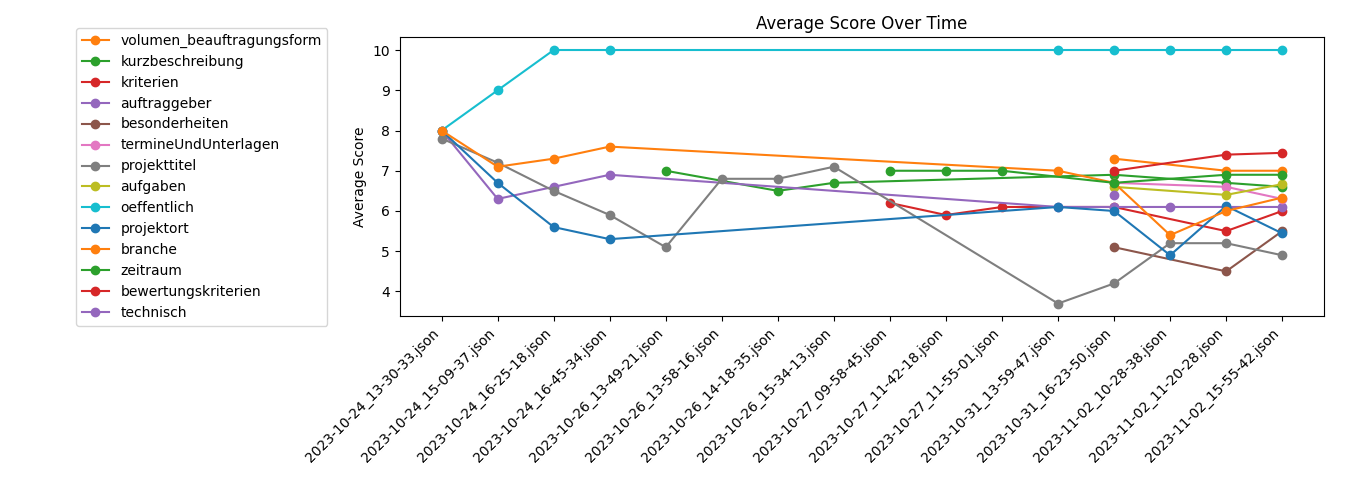
\includegraphics[width=0.8\textwidth]{figures/03_Prompt_Evaluierung.png}
    \caption{Visualisierung der durchschnittlichen Promptqualität im Laufe der Zeit}
    \label{fig:03_Prompt_Evaluierung}    % \ref{fig:03_Prompt_Evaluierung}
    \end{figure}

\subsection{Datenschutz}
Das übermitteln und verarbeiten von Personenbezogenen Daten ist in Deutschland nur mit Ausdrücklicher Genehmigung der 
entsprechenden Person zulässig. Es ist unklar inwiefern das Übermitteln der Daten aus den Dokumenten über die openAI 
API hierunter einzustufen ist. Offiziell heißt es, dass die Daten, welche über die API geteilt werden, nicht zu 
Trainingszwecken genutzt werden. Da die Server von openAI allerdings in den USA liegen gestalten sich Probleme mit 
europäischen Datenschutzrecht. Als Lösung wurde die Umstellung auf Azure in Betracht gezogen, da die Server auf europäischen 
Boden stehen und damit zumindest nach europäischen Recht Datenschutzkonform sind. Ein großer Nachteil von Azure ist aber, 
dass man für das erstellen der Vektordatenbank auf 16 Inputs beschränkt ist, während openAI hier keine Einschränkungen vorgibt. 
Größere Dokumente können leicht auf 1 Input pro Seite kommen, was ein Einbetten von Dokumenten ab 20 Seiten verhindert.
Um das Problem zu lösen habe ich statt die vorgegebene Embedding-Methode zu verwenden eine eigene Methode erstellt, 
welche die Dokumente bzw. die Inputs auf mehrere Listen mit einer Größe kleiner gleich 16 aufteilt. Anschließend werden 
die einzelnen Listen über eine REST API zu embeddings umgewandelt und anschließend wieder zusammengesetzt. Am ende wird eine 
Collection mit den Embeddings, den Dokumenten und entsprechenden Metadaten erstellt, welche zentral in einem VectorDataManager 
zur Verfügung gestellt wird. Gegen diese Collection können anschließend Abfragen wie Similarity-Searches durchgeführt werden.

\section{Ergebnisse und Erfahrungen}